\chapter{Driven cavity problem}
The driven cavity problem consists in a two-dimensional cavity with an incompressible fluid. The upper wall of the cavity moves at a given velocity, as shown in figure \ref{DrivenCavityImg}. The aim of the problem is to obtain the distribution of velocities inside the cavity.
\begin{figure}[h]
	\centering
	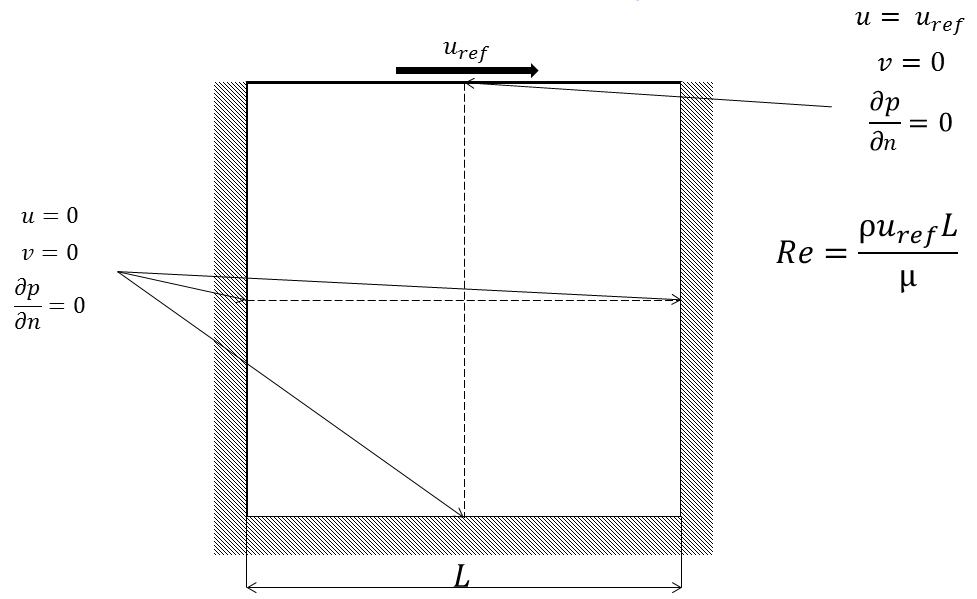
\includegraphics[scale=0.5]{DrivenCavity/DrivenCavity}
	\caption[General scheme of the driven cavity problem]{General scheme of the driven cavity problem. Extracted from \cite{CTTCa}}
	\label{DrivenCavityImg}
\end{figure}

\section{Discretization}
The domain is discretized, as explained in section \ref{FSMDiscretization}, using the staggered meshes. To do so, the volume is divided using a Cartesian grid, with the following characteristics:
\begin{table}[]
	\centering
	\begin{tabular}{ |c|c|c|c|c|c|c| }
		\hline
		$N$ & $M$ & $L$ & $\rho$ & $u_{ref}$ & $\mu$ & $\delta$ \\ \hline
		$100$ & $100$ & $1$ & $1$ & $1$ & $\frac{1}{Re}$ & $10^{-5}$ \\ \hline
	\end{tabular}
\caption{Numerical parameters of the driven cavity problem}
\end{table}

The length of the cavity $L$, the density $\rho$, the velocity $u_{ref}$ and the viscosity $\mu$ are chosen in order to have a non-dimensional problem. 

\section{Boundary conditions}
It is necessary to impose the conditions defined by figure \ref{DrivenCavityImg}. There are two types of conditions: the prescribed velocity, and the boundary layer conditions. The last ones are defined by assuming that the pressure gradient normal to the wall is 0. For example, in the left wall:
\begin{equation}
	\frac{\partial p}{\partial x}\approx\frac{p_{E}-p_{P}}{\Delta x}=0
\end{equation}
\begin{equation}
p_{P}=p_{E}
\end{equation}
These boundary layer conditions modify the discretization coefficients in the boundary nodes. The coefficients are listed in table \ref{DCBoundaryCoefficients}.
\begin{table}[h]
	\centering
	\begin{tabular}{ |c|c|c|c|c| }
		\hline
		Coefficients & Top & Bottom & Left & Right \\ \hline
		$a_{E}$ & 1 & 0 & 1 & 0 \\ \hline
		$a_{W}$ & 0 & 0 & 0 & 1 \\ \hline
		$a_{N}$ & 0 & 1 & 0 & 0 \\ \hline
		$a_{S}$ & 0 & 0 & 0 & 0 \\ \hline
		$a_{P}$ & 1 & 1 & 1 & 1 \\ \hline
	\end{tabular}
\caption{Discretization coefficients in the boundary}
\label{DCBoundaryCoefficients}
\end{table}

The condition of prescribed velocity in the walls is achieved with the following conditions:
\begin{itemize}
	\item $R\left(\vec{v}\right)=0$ in the top
	\item $R\left(\vec{v}\right)=0$ in the bottom wall
	\item $R\left(\vec{v}\right)=0$ in the left wall
	\item $R\left(\vec{v}\right)=0$ in the right wall
\end{itemize}
And the prescribed velocities are:
\begin{itemize}
	\item $u=u_{ref}$, $v=0$ in the top
	\item $u=0$, $v=0$ in the bottom wall
	\item $u=0$, $v=0$ in the left wall
	\item $u=0$, $v=0$ in the right wall
\end{itemize}

\section{Algorithm}
\begin{figure}[H]
	\centering
	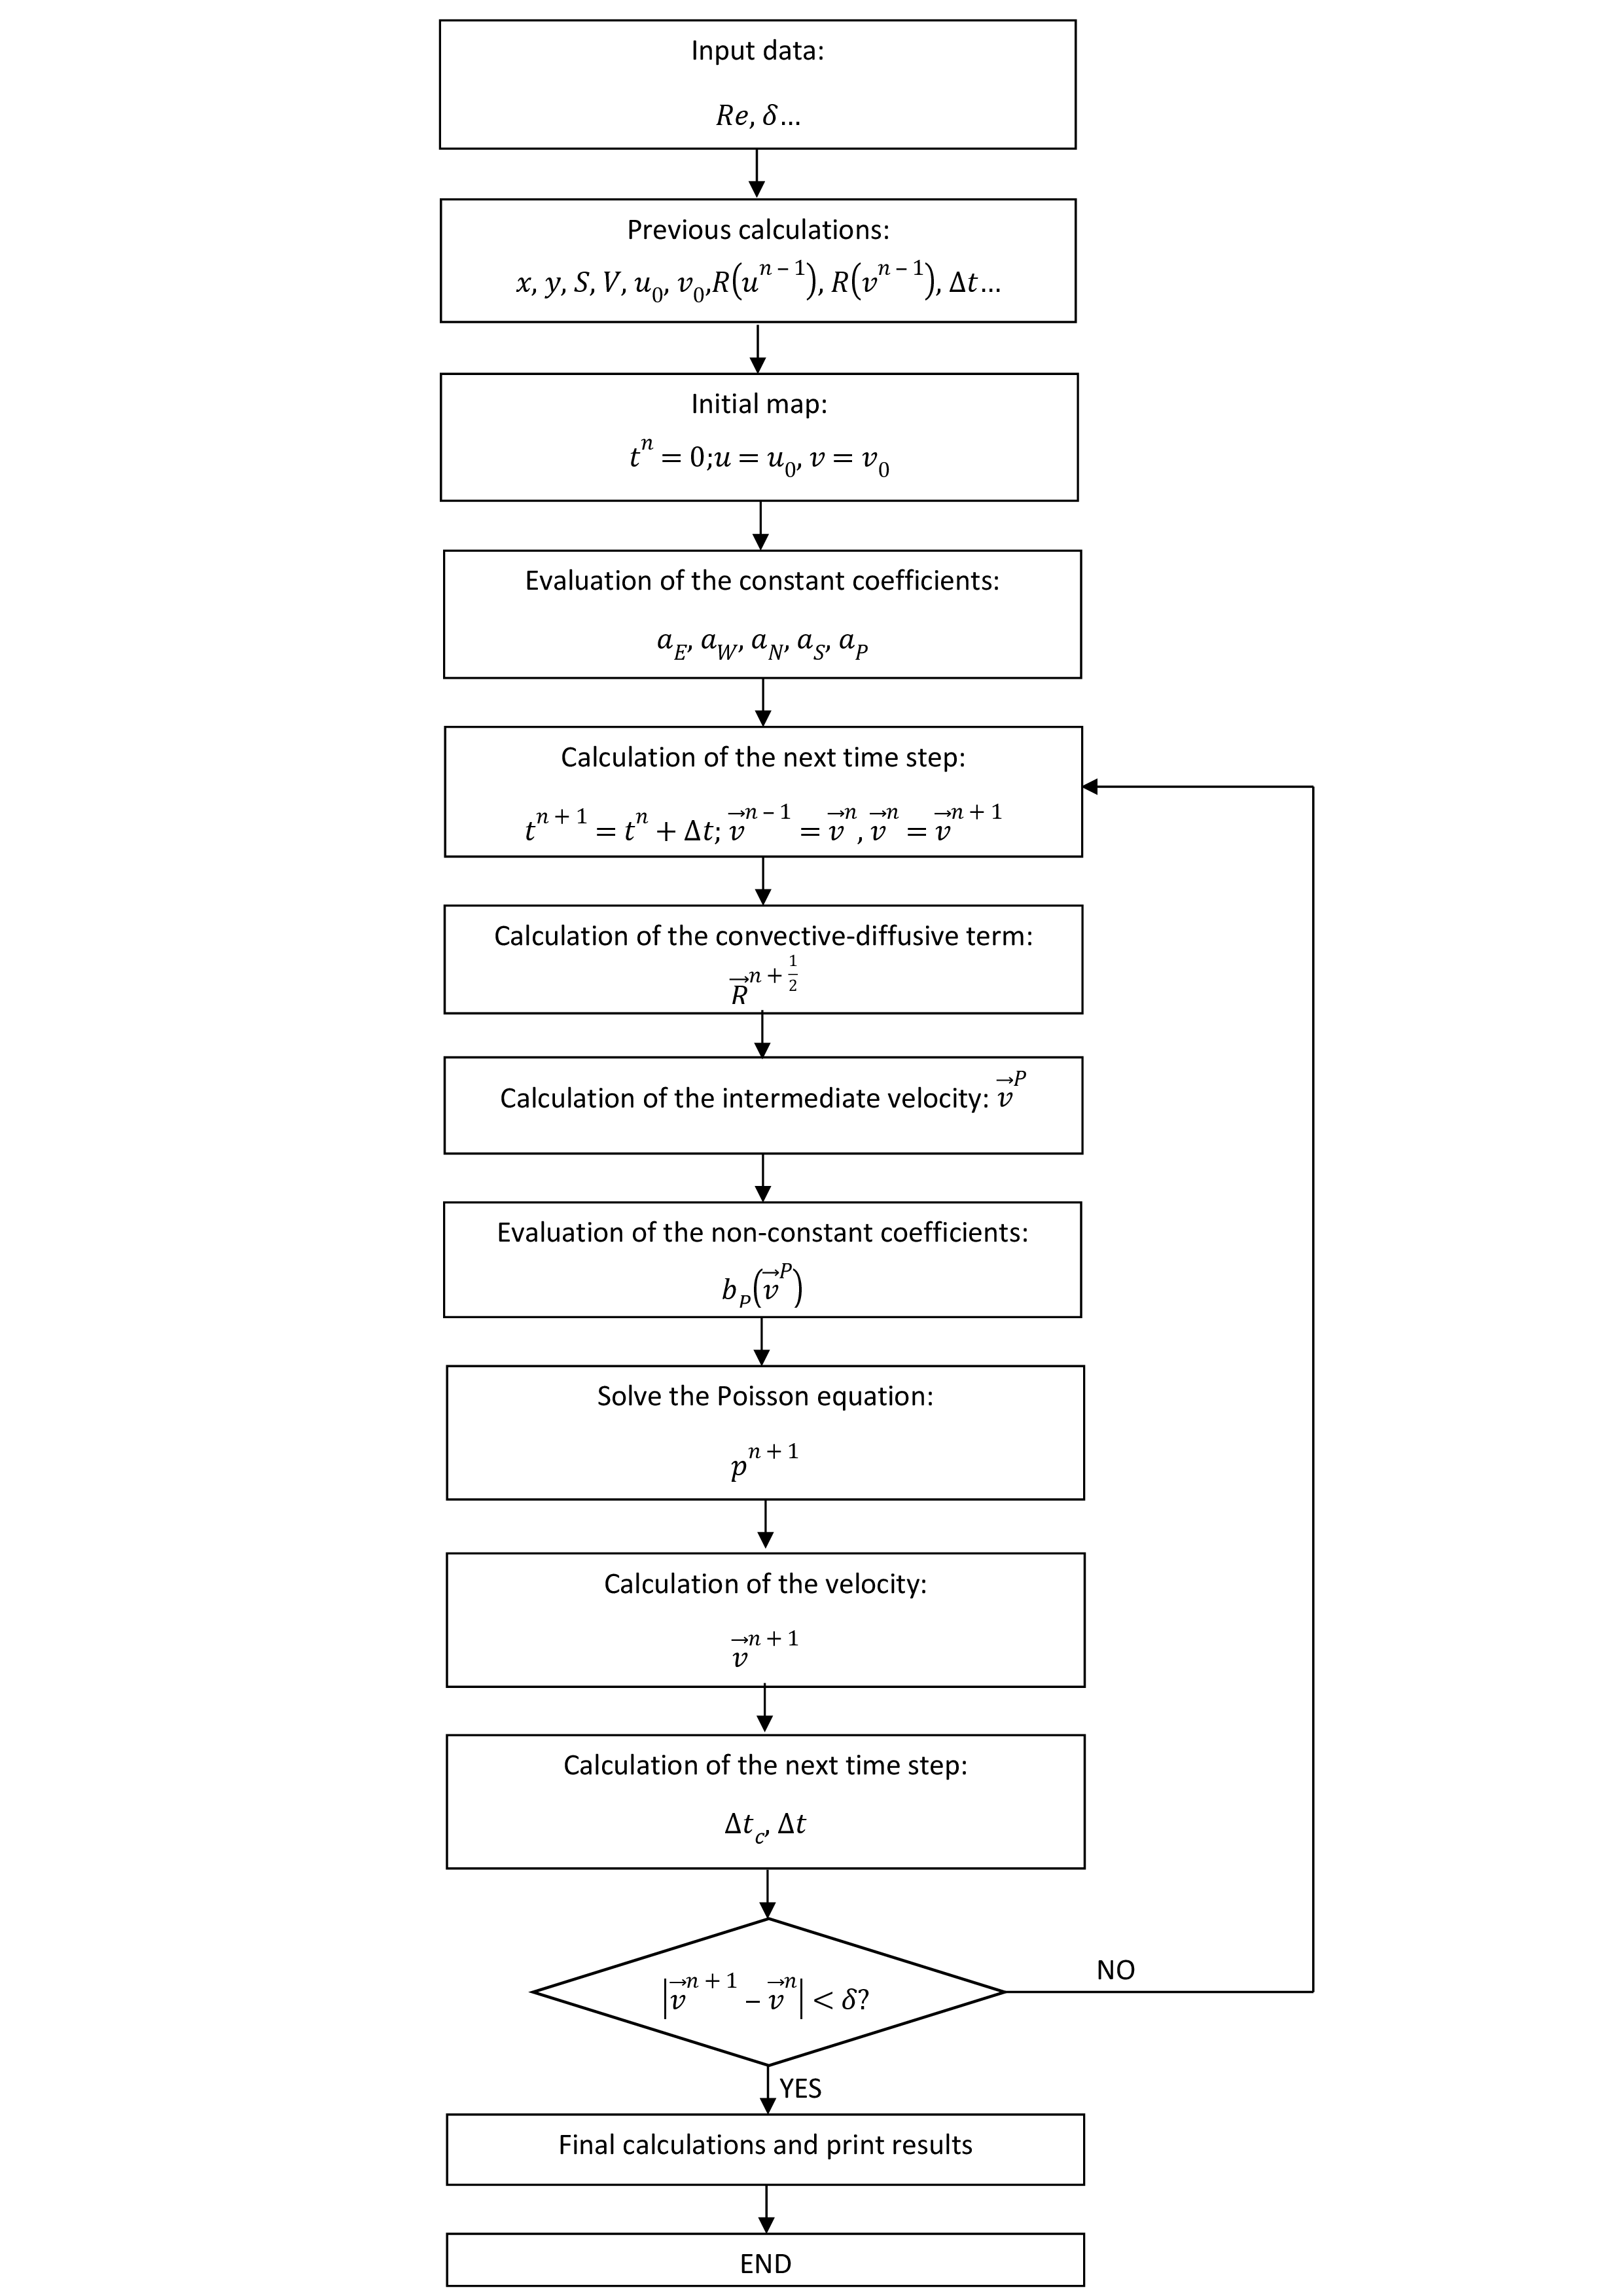
\includegraphics[scale=0.169]{DrivenCavity/algorithm}
\end{figure}
The simulation of the driven cavity problem ends when it reaches a steady state.

\section{Results}
